%%%-----------------------------------------------------------------------------
\section{Idealised axial passages}
\label{sec:idealAxial}
%%%-----------------------------------------------------------------------------

For purely axial machines, the flow on the meridional surface can be
represented in a 2D plane by using the \emph{conformal} (\ie
maintaining the relative angles) transformation
\begin{align*}
  dx &= dm & dy &= r d \theta
\end{align*}
This procedure is illustrated in figure \ref{fig:meridionalCut} for an
axial machine. In an axial machine, especially when the blade spacing
is small with respect to the radius, the flow on a meridional surface
can be approximated by the flow in a linear \emph{cascade}, \ie a
periodic linear arrangement of airfoils, resulting from unfolding the
cut of the surface with the blades.
\begin{figure}[!h]
  \centering
  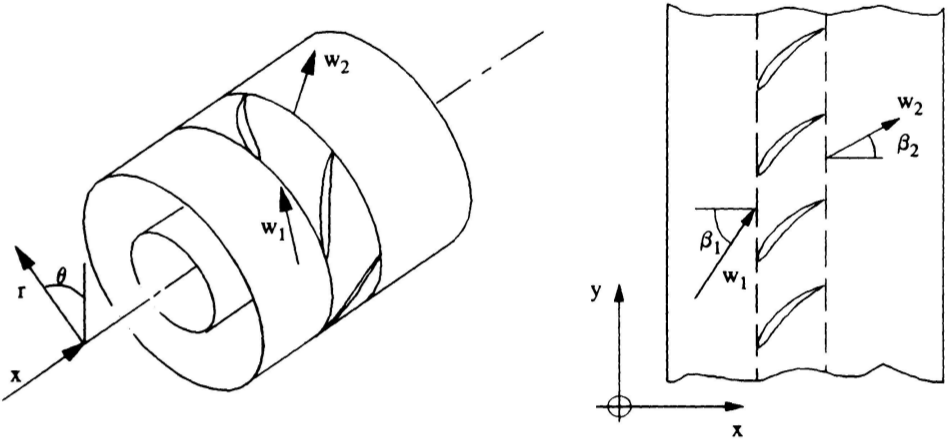
\includegraphics[width=0.8\textwidth]{meridionalPlaneUnfolded.png}
  \caption{Cascade as a simplification of a meridional stream surface.}
  \label{fig:meridionalCut}
\end{figure}
In case the hub radius is large with respect to the shroud radius, the
radial varation of the conditions along the span is small and we can
perform a \emph{pitch-line} analysis, \ie an analysis at the center of
the span, to predict the global performance. In the more general case,
we can apply this analysis for several radial stations, thereby
mapping the spanwise variation of the operating conditions. An
additional radial equation will then be used to link the conditions
along the span. In case of a rotating blade row, the circumferential
speed of the linear cascade is obviously $\fVel = \rot R$ with R the
radius of the cut.


\subsection{Geometric definition of a cascade}
\label{sec:cascadeGeometry}

\begin{figure}[!h]
  \centering
  \begin{subfigure}{0.44\textwidth}
    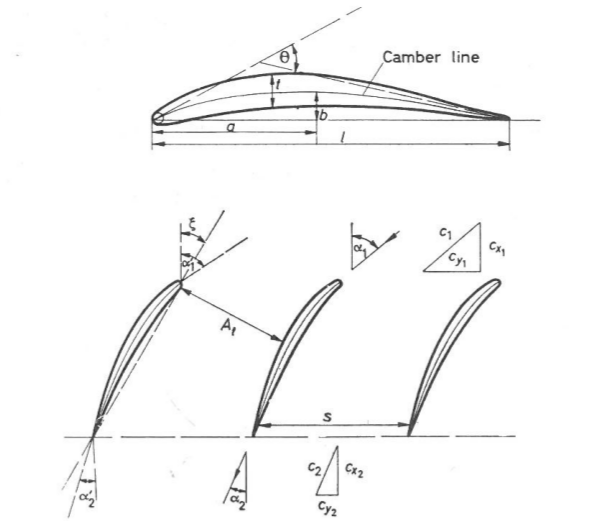
\includegraphics[width=\textwidth]{cascadeTerminology_howell_horlock.png}
    \caption{Geometry definitions following Howell}
    \label{fig:cascadeGeometry}
  \end{subfigure}
  \begin{subfigure}{0.55\textwidth}
    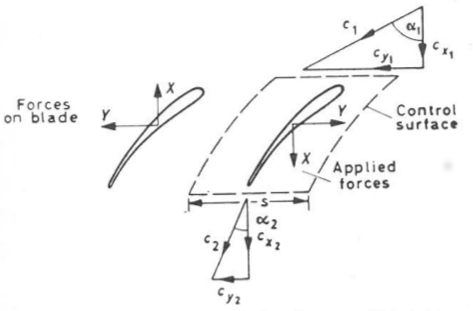
\includegraphics[width=\textwidth]{cascadeControlVolume_horlock.png}
    \caption{Control volume}
    \label{fig:cascadeControlVolume}
  \end{subfigure}
  \caption{Cascade parameter definitions by Horlock \cite{Horlock}.
    Flow velocity marked with $c$, chord $l$ and stagger by
    $\xi$. Meridional direction aligned with x and tangential direction with y}
  \label{fig:cascadeDefinition}
\end{figure} 
Referring to figure \ref{fig:cascadeDefinition}, a linear cascade is
determined first of all by the blade geometry, typically defined in
terms of a \emph{camber line} (central fiber) and a \emph{thickness
  distribution} $t$ around it. The following global parameters are
often used:
\begin{itemize}
\item the \emph{chord} $\chord$, \ie the distance between leading to
  trailing edge;
\item the \emph{camber angle}, \ie the difference between in- and
  outlet blade angle $\camberAngle = \bladeAngle_1 - \bladeAngle_2$;
\item the position $a$ and height $b$ of the maximum camber;
\end{itemize}
The cascade is further characterised by the placement of the blades,
namely
\begin{itemize}
\item the \emph{stagger angle} \stagger,\ie the angle between the
  blade chord line and the axial direction;
\item the blade tangential spacing or \emph{pitch} \pitch.
\end{itemize}
The non-dimensional cascade geometry is then characterised by the
stagger angle \stagger~ and the \emph{solidity} $\solidity =
\chord/\pitch$ or alternatively its inverse, the \emph{pitch-to-chord
  ratio}.  

\subsection{Relative flow in cascades}
\label{sec:cascadeStationary}

In order to compute the forces on the profile, a control volume is
defined in the stationary cascade as illustrated in figure
\ref{fig:cascadeControlVolume}. In this figure, $x$ corresponds to the
meridional direction $m$, whereas $y$ corresponds to the tangential
direction $u$.  

The flow in a cascade is quite different from that around an isolated
airfoil. First of all, there is a clear distinction between flow
conditions before (1) and after (2) the cascade. Due to the flow
deflection, it is not clear which velocity should be chosen as
reference. Finally, the forces acting on the blades are impacted by
the interference with the adjacent blades in the cascade.

The flow angles $\aFlowAngle_1$ and $\aFlowAngle_2$ do not correspond
to the blade metal angles $\bladeAngle_1$ and $\bladeAngle_2$. As in
isolated airfoil theory, the difference at the inlet is called
\emph{incidence}
\begin{align*}
  \incidence = \aFlowAngle_1 - \bladeAngle_1
\end{align*}
An alternative characterisation of the inflow angle is the \emph{angle
  of attack}, corresponding to the difference with respect to the
stagger angle, or the angle between the flow and the chord line:
\begin{align*}
  \angleOfAttack = \aFlowAngle_1 - \stagger
\end{align*}
The difference of the flow angle with the blade angle at the outlet is
called the \emph{deviation}
\begin{align*}
  \deviation = \aFlowAngle_2 - \bladeAngle_2
\end{align*}
characterising the departure from perfect guidance by the cascade.
Finally, the action of the cascade is determined by the
\emph{deflection} or \emph{turning angle}
\begin{align*}
  \deflection = \aFlowAngle_2 - \aFlowAngle_1
\end{align*}
The force exerted by the blade on the flow is found by the momentum
balance the control volume shown in figure
\ref{fig:cascadeControlVolume}:
\begin{align*}
  \force_m &= \pitch (\pres_2 - \pres_1) +
  \mFlow \left(\aVel_{m2} - \aVel_{m1}\right) = \pitch (\pres_2 - \pres_1) \\
  \force_\fVel &= \mFlow \left(\aVel_{\fVel 2} - \aVel_{\fVel 1}\right)
\end{align*}
Since the flow is incompressible, conservation of mass imposes that
$\vel_{m1} = \vel_{m2}$. We then define the averaged flow velocity
$\overline \aVelV = \aVelV_1 + \aVelV_2$. In the absence of losses,
Bernoulli's equation tells us the total pressure of the flow should
remain constant. Projecting the force on the average velocity between
in- and outlet, we find
\begin{align*}
  \force_m ~ \overline{\aVel_{m}} + 
  \force_\fVel ~ \overline{\aVel_{\fVel }} &=
  \vFlow \left( \pres_2 - \pres_1\right) + 
  \mFlow ~\frac{\aVel_{m2}^2 - \aVel_{m1}^2}{2} + 
  \mFlow ~\frac{\aVel_{\fVel 2}^2 - \aVel_{\fVel 1}^2}{2} \\
  &= \mFlow \frac{\sPres{2} - \sPres{1}}{\dens} = \mFlow \frac{\Delta_{12}^l \sPres{}}{\dens}
\end{align*}
Note that the viscous force $\force_m$ opposes the flow and therefore,
$\Delta_{12}^l \sPres{} \leq 0$. With the suffix $l$ we indicate this
concerns the total pressure loss in the cascade. This loss is only
zero if the force is orthogonal to the arithmetic average of in- and
outflow velocity. This average flow velocity therefore generalizes the
freestream velocity for profiles to cascade flows\footnote{Without
  friction, the force on an isolated airfoil consists of lift and is
  orthogonal to the free-stream velocity.}. The action of the cascade
is then characterised by the lift \lift~ and drag force \drag~defined
with respect to this average velocity:
\begin{align*}
  \lift &=  
  \force_m \frac{\bar \aVel_\fVel}{\bar \aVel} -
  \force_\fVel \frac{\bar \aVel_m}{\bar \aVel}  &
  \drag &= -
  \force_m \frac{\bar \aVel_m}{\bar \aVel} -
  \force_\fVel \frac{\bar \aVel_\fVel}{\bar \aVel}
\end{align*}
Note that these are defined with respect to the blade.  The total
enthalpy is preserved across the blade row, such that
\begin{align*}
  \Delta_{12} \sEnth{} = \heatCapV \Delta_{12} T + \frac{\Delta_{12}^l
    \sPres{}}{\dens} = 0
\end{align*}
and therefore the total pressure loss is converted in thermal energy:
\begin{align*}
  \Delta_{12} T = - \frac{\Delta_{12}^l \sPres{}}{\dens \heatCapV}
\end{align*}
The static pressure difference across the cascade is
\begin{align*}
  \Delta_{12} \pres &= \frac{1}{2} \dens
  \left(\aVel_{1}^2 - \aVel_{2}^2\right) + \Delta_{12}^l \sPres{} \\
  &= \frac{1}{2} \dens
  \left(\aVel_{\fVel 1}^2 - \aVel_{\fVel 2}^2\right) + \Delta_{12}^l \sPres{} \\
  &= \frac{1}{2} \dens \aVel_m^2~\left(\tan^2 \alpha_1 - \tan^2
    \alpha_2\right) + \Delta_{12}^l \sPres{}
\end{align*}
Neglecting the total pressure loss, we can see that the pressure
increase equals the diffusion of the tangential velocity
$\aVel_\fVel$. Cascades that reduce the tangential component of the
velocity, or equivalently decrease the flow angle will diffuse kinetic
energy to increase static pressure and are found in pumps, fans or
compressors. Conversely, an increase of the flow angle a priori
correspond to an accelerating cascade, found in turbines.

% \subsection{Efficiency of a diffusing cascade}

% \begin{figure}[!h]
%   \centering
%   \begin{subfigure}{0.5\textwidth}
%     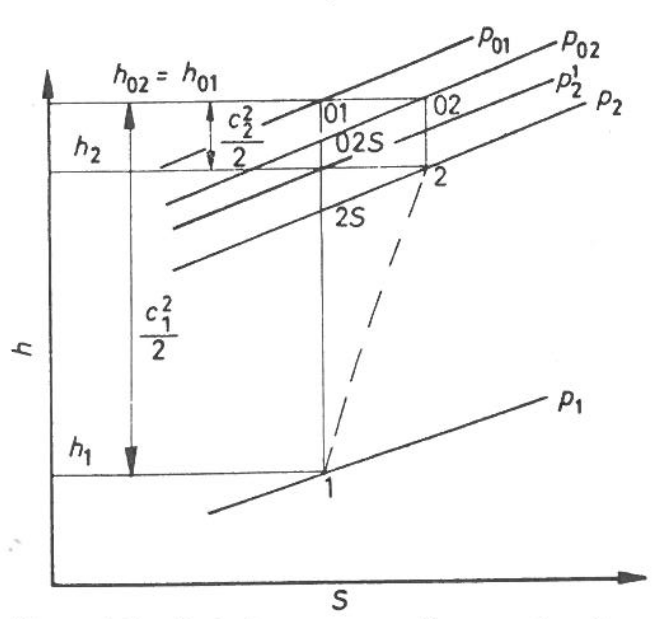
\includegraphics[width=\textwidth]{compressorStatorMollier_horlock.png}
%     \caption{Pump/fan cascade}
%   \end{subfigure}
%   % \begin{subfigure}{0.5\textwidth}
%   %   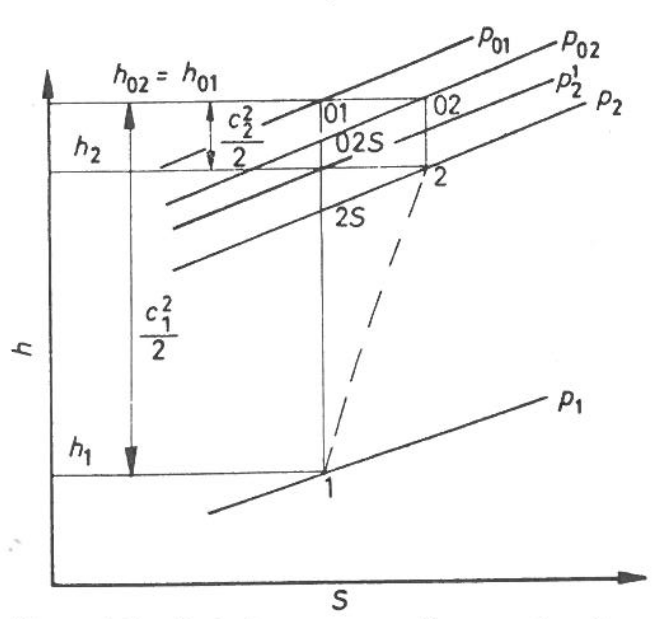
\includegraphics[width=\textwidth]{compressorStatorMollier_horlock.png}
%   %   \caption{Turbine cascade}
%   % \end{subfigure}
%   \caption{Thermodynamic state diagram for the flow in a stationary
%     cascade. From Horlock \cite{horlock}. Velocity is denoted by $c$.}
%   \label{fig:mollierHsStator}
% \end{figure}
% The Mollier enthalpy-entropy or $\enth-\entr$ diagram, shown in figure
% \ref{fig:mollierHsStator} for a diffusing cascade allows us to define
% measures for the efficiency. At the inlet of the cascade, we are at
% the point $(\enth_1,\entr_1)$:
% \begin{align*}
%   \enth_1 &= \heatCapV \left(\temp_1 - \temp^\ast\right) + \frac{\pres_1 - \pres^\ast}{\dens} \\
%   \entr_1 &= \heatCapV \ln\left(\temp_1/\temp^\ast\right)
% \end{align*}
% which is located on the isobar $\pres = \pres_1$. The flow has a
% velocity $\aVel_1$, and therefore the total enthalpy consists of the
% static enthalpy and the kinetic energy:
% \begin{align*}
%   \sEnth{1} &= \enth_1 + \frac{1}{2} \aVel^2_1 
% \end{align*}
% The point $(\sEnth{1},\entr_1)$ is located on the total pressure
% isobar $\pres = \sPres{1}$. Going to the outlet, the total enthalpy is
% conserved, \ie $\sEnth{2} = \sEnth{1}$, however we have lost a total
% pressure of $- \Delta_{12}^l \sPres{}$, and therefore the total
% conditions are located on the isobar $\pres = \sPres{1} +
% \Delta_{12}^l \sPres{}$, giving entropy $\entr_2$. Finally, the static
% conditions at the outlet are found by subtracting the kinetic energy
% from the total enthalpy $\enth_2 = \sEnth{2} - \frac{1}{2} \aVel_2^2$,
% located on the isobar $\pres = \pres_2$.

% The intersections of the isobar $\pres_2$ with $\entr=\entr_1$ then
% give us the static enthalpy rise for the same pressure rise for an
% isentropic diffusion, \ie if no losses would have been
% encountered. The \emph{static to static isentropic efficiency} is then
% \begin{align*}
%   \eff_{ss} 
%   &
%   = \frac{\Delta_{12}^s \enth}{\Delta_{12} \enth} = \frac{\enth_{2s} - \enth_1}{\enth_2 - \enth_1} 
%   = \frac{\pres_2 - \pres_1}{\frac{1}{2} \left(\aVel_1^2 - \aVel_2^2\right)}
% \end{align*}
% indicating that this efficiency quantifies the part of the kinetic
% energy that was effectively converted in pressure rise and is
% therefore equal to the \emph{diffusion efficiency} 
% \begin{align*}
%   \eff_D 
%   &
%   = \frac{\pres_2 - \pres_1}{\pres^\prime_2 - \pres_1} 
%   = \frac{\pres_2 - \pres_1}{\frac{1}{2} \left(\aVel_1^2 - \aVel_2^2\right)}
% \end{align*}

\subsection{Non-dimensional performance of the stationary cascade}
\label{sec:cascadeNonDimensional}

We now determine the minimum number of parameters that govern cascade
performance using the similarity analysis. For a given airfoil shape,
the forces, pressure differences, \ldots are determined by the
\begin{itemize}
\item the cascade parameters: pitch \pitch, chord \chord~ and stagger
  angle \stagger;
\item the flow is characterised by velocity \aVel~and flow angle
  \aFlowAngle\footnote{As the fluid is incompressible the absolute
    value of the pressure is irrelevant};
\item the fluid properties, namely density $\dens$ and dynamic
  viscosity $\dynVisc$.
\end{itemize}
The performance of the cascade is characterised by either the aerodynamic forces
\begin{align*}
  \lift &= \lift(\chord,\pitch,\stagger,\alpha,\aVel,\dens,\dynVisc) & 
  \drag &= \drag(\chord,\pitch,\stagger,\alpha,\aVel,\dens,\dynVisc) 
\end{align*}
or more conveniently the total pressure loss and the deflection
\begin{align*}
  \Delta_{12}^l \sPres{} &= f(\chord,\pitch,\stagger,\alpha,\aVel,\dens,\dynVisc) &
  \deflection &= f(\chord,\pitch,\stagger,\alpha,\aVel,\dens,\dynVisc) 
\end{align*}
These are relations between 8 parameters; since there are 3
fundamental dimensions (length, time and mass), the relations
describing cascade performance involve each time 5 parameters. We need
to non-dimensionalize three performance parameters. The lift and drag
are nondimensionalised by the kinetic energy associated to the average
velocity:
\begin{align*}
  \liftCoeff &= \frac{L}{\frac{1}{2} \dens \bar \aVel^2~\pitch} & 
  \dragCoeff &= \frac{D}{\frac{1}{2} \dens \bar \aVel^2~\pitch}
\end{align*}
The total pressure loss is non-dimensionalised by a dynamic pressure
to the \emph{loss coefficient}
\begin{align*}
  \lossCoeff = - \frac{\Delta_{12}^l \sPres{}}{\frac{1}{2} \dens \aVel^2}
\end{align*}
Notice that we did not specify which velocity is used to
non-dimensionalize the loss. Traditionally the upstream value
$\aVel_1$ is used for pumps or fans whereas the downstream value
$\aVel_2$ is typically used for turbines.  In terms of the independent
parameters, the geometry is characterised by the solidity $\sigma =
\chord/\pitch$, whereas the flow conditions are characterised by the
Reynolds number $Re=\dens \vel \chord/\dynVisc$. Hence we can
characterise the cascade by measuring the dependence
\begin{align*}
  \liftCoeff &= \liftCoeff(\solidity,\stagger,\alpha,Re) & 
  \dragCoeff &= \dragCoeff(\solidity,\stagger,\alpha,Re)
\end{align*}
or alternatively
\begin{align*}
  \lossCoeff &=   \lossCoeff(\solidity,\stagger,\alpha,Re) &
  \deflection &= \deflection(\solidity,\stagger,\alpha,Re)
\end{align*}

If the blades are sufficiently spaced, one can use the lift-drag
characteristics of the isolated airfoil.  Due to the large set of
parameters, the obtention of true cascade performance data is rather
involved. We will not go into the correlations that have been proposed
to provide priori estimations of the performance. A well-known example
of an actual data base are the NACA studies on compressor cascades
based upon the NACA 65 profile family, reported by Herrig \etal
\cite{NACA-TN-3916}. Figure \ref{fig:naca65Perfo} shows a sample
result of these measurements.
\begin{figure}[!h]
  \centering
  \begin{subfigure}{0.52\textwidth}
    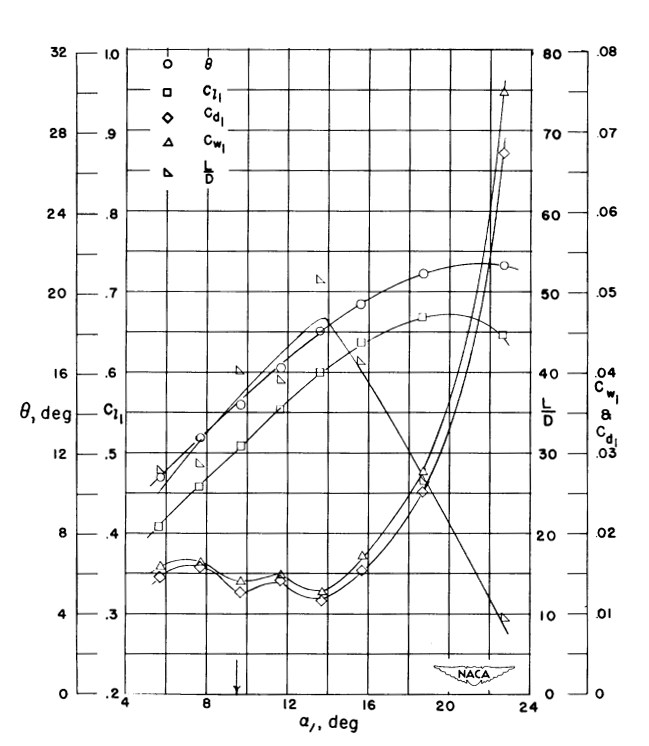
\includegraphics[width=\textwidth]{naca65_810_sol1_beta45.png}
    \caption{Cascade performance diagram for constant inflow angle
      $\aFlowAngle_1$ as a function of incidence $\incidence$.}
    \label{fig:naca65Perfo_polar}
  \end{subfigure}
  \begin{subfigure}{0.47\textwidth}
    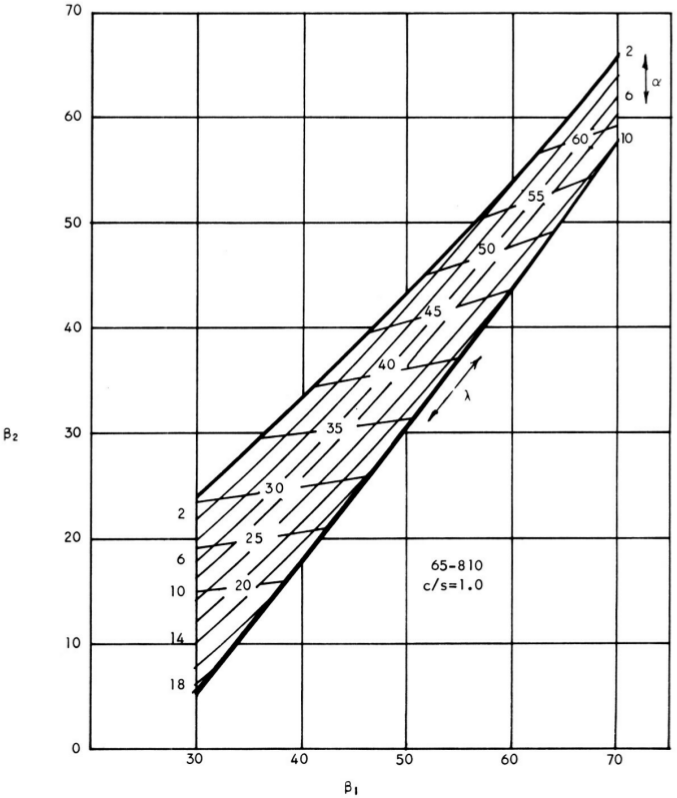
\includegraphics[width=\textwidth]{naca65_810_sol1_mellor.png}
    \caption{Mellor diagram $\alpha_2$ vs $\alpha_1$.}
    \label{fig:naca65Perfo_Mellor}
  \end{subfigure}
  \begin{subfigure}{0.47\textwidth}
    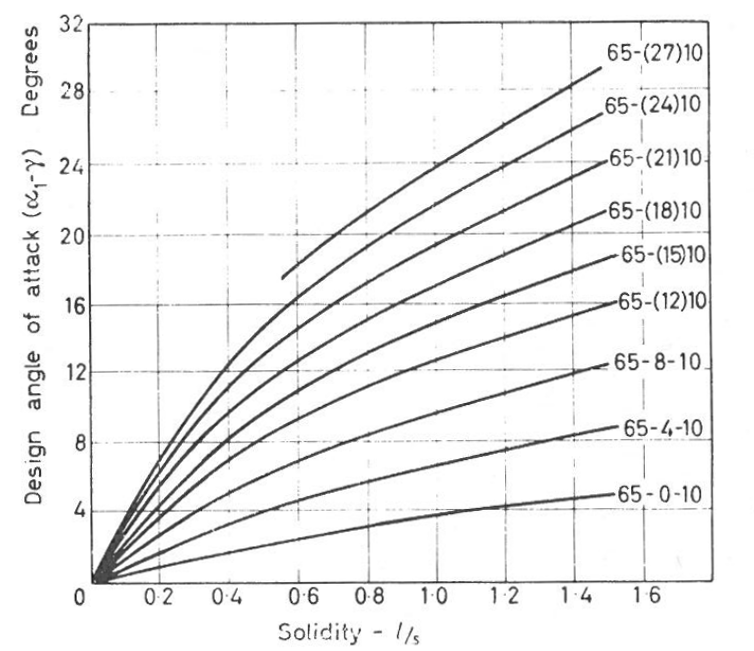
\includegraphics[width=\textwidth]{naca65_optimalIncidence.png}
    \caption{Optimal incidence for NACA65 cascades.}
    \label{fig:naca65Perfo_incidence}
  \end{subfigure}
  \caption{Performance of NACA65(8)10 cascades at solidity
    $\solidity=1$. Diagram showing turning angle $\deflection$, $C_L$,
    $C_D$ as a function of the angle of attack (noted by $\alpha_i$)
    for $\aFlowAngle_1 = 45°$ (left) from Herrig \etal
    \cite{NACA-TN-3916}; Mellor diagram linking flow angles
    \cite{Mellor57}; optimal incidence for NACA65 family.}
  \label{fig:naca65Perfo}
\end{figure}
It should be noted that the lift-drag diagrams are provided for a
fixed \emph{flow angle} $\aFlowAngle_1$, and provide variations as a
function of angle of attack $\angleOfAttack = \aFlowAngle_1 -
\stagger$. This means that effectively the stagger is varied instead
of the flow angle and therefore this graph does not correspond to a
given cascade.

Mellor \cite{Mellor57} reorganised the data, allowing to identify
stagger and incidence from the in- and outflow angle. An example of
such a map is shown in figure \ref{fig:naca65Perfo_Mellor}. This diagram
also shows the positive and negative incidence stall line, \ie the
angles corresponding to a 50\% increase of the loss coefficient with
respect to the minimum. Finally, Herrig \etal plotted optimal
incidence for all NACA65 cascades. For a given deflection and inlet
flow angle, the Mellor plots allow to identify the different
alternative cascade configurations, which can then be checked for
optimal incidence and classified in terms of loss coefficient.

\subsection{Moving cascade}
\label{sec:cascadeMoving}

Now we look at a cascade moving with velocity $\fVel$. As the frame is
moving linearly with respect to the absolute frame, the governing
equations in the relative frame are the same as in the absolute
frame. We can therefore directly apply the results of section
\ref{sec:cascadeStationary} to the relative velocities. This means
that the performance maps from section \ref{sec:cascadeNonDimensional}
can be directly used to predict forces and losses in the relative
frame. The forces can determined from the relative velocities:
\begin{align*}
  \force_m &= P (\pres_2 - \pres_1) \\
  \force_\fVel &= \mFlow \left(\rVel_{\fVel 2} - \rVel_{\fVel 1}\right) 
  = \mFlow \left(\aVel_{\fVel 2} - \aVel_{\fVel 1}\right) 
\end{align*}
The power transferred from the blades to the flow is given by
\begin{align*}
  \power 
  &= \force_\fVel \fVel 
  = \mFlow \left(\fVel \rVel_{\fVel 2} - \fVel \rVel_{\fVel 1}\right) 
  = \mFlow 
  \left(
    \frac{\rVel_1^2 - \rVel_2^2}{2} + 
    \frac{\aVel_2^2 - \aVel_1^2}{2} \right)
\end{align*}
Also the loss of total pressure in the relative frame is
\begin{align*}
  \Delta_{12}^l \sPres{} &= \forceV \cdot \overline{\rVelV}
\end{align*}
hence we have
\begin{align*}
  \pres_1 + \frac{\dens \rVel_1^2}{2} = 
  \pres_2 + \frac{\dens \rVel_2^2}{2} - \Delta_{12}^l \sPres{}
\end{align*}
and therefore
\begin{align*}
  \power &= \mFlow \left( \pres_2 - \pres_1 + \frac{\aVel_2^2}{2} -
    \frac{\aVel_1^2}{2} \right)
  - \mFlow \frac{\Delta_{12}^l \sPres{}}{\dens} = \mFlow \frac{\Delta_{12}^s \sPres{}}{\dens} - \mFlow \frac{\Delta_{12}^l
    \sPres{}}{\dens}
\end{align*}
This interesting result indicates that the useful work consists of
diffusion/acceleration in the relative frame, \ie pressure difference
$\Delta_{12} p$, and a change in the absolute kinetic energy. Moreover, the
total pressure loss computed in the relative frame, directly
translates to the absolute frame.

\subsection{Non-dimensional stage parameters}

Assuming geometric similarity, fixing inlet flow angle, stagger angle
and solidity, the useful work and loss are function of axial velocity
(or alternatively flow rate), rotation velocity, chord, density and
viscosity. Therefore, we have relations between 3 non-dimensional
parameters. We define the (stage) \emph{flow} coefficient \flowCoeff~
and the \emph{load} or \emph{head} coefficient \headCoeff~ as
\begin{align*}
  \flowCoeff &= \frac{\aVel_m}{\fVel} &
  \headCoeff &= \frac{\Delta_{12}^s \sPres{}}{\dens \fVel^2}
\end{align*}
and then the load coefficient is a function of flow coefficient and
Reynolds number
\begin{align*}
  \headCoeff &= f(\flowCoeff,Re)
\end{align*}

A final important non-dimensional parameter is the so-called specific
speed, which relates the rotation speed with respect to flow rate
$\vFlow$ and total enthalpy rise $\Delta \sPres{}/\dens$. The
dimensions of $\specificSpeed$ are given by
\begin{align*}
  [\specificSpeed] 
  &= \left[\rot \right] \cdot \left[\vFlow\right]^a \cdot \left[\frac{\Delta \sPres{}}{\dens}\right]^b 
  %&= \frac{1}{t^{\ast}} \cdot \left(\frac{L^{\ast 3}}{t^{\ast}}\right)^a \cdot \left(\frac{L^{\ast 2}}{t^{\ast 2}}\right)^b
\end{align*}
which is non-dimensional if the powers of the reference time $t^\ast$ and
length scale $L^\ast$ are zero:
\begin{align*}
  t^\ast~&:~ &- a - 2b =  1 \\
  L^\ast~&:~ & 3a + 2b = 0 \\
\end{align*}
and therefore $a=1/2$ and $b=-3/4$. Hence 
\begin{align*}
  \specificSpeed = \frac{\rot \sqrt{\vFlow}}{\left(\frac{\Delta \sPres{}}{\dens}\right)^{3/4}}
\end{align*}

\subsection{Degree of reaction}


An important design parameter is the \emph{degree of reaction}. It is
defined as the part of the pressure rise/drop realised in the rotor to
the total pressure rise. The static pressure difference also
corresponds to the enthalpy change for an isentropic process.
\begin{align*}
  \reaction = 
  \frac{\Delta_{12} \pres}{\Delta_{12}^s \sPres{}} = 
  \frac{\Delta_{12}^s \enth}{\Delta_{12}^s \tEnth}
\end{align*}

\subsection{Pump/fan stage} 

Typically, the pump/fan stage consists either of a single rotor or a
combination of rotor and stator. In order to transfer work, the rotor
has to deflect the flow in the direction of the rotation. A purely
axial inflow is therefore a relatively good solution, and then
\begin{align*}
  \power = \mFlow \fVel \aVel_{\fVel 2} 
\end{align*}
The tangential component of the absolute velocity $\aVel_{\fVel 2}$ not
only determines work, but also introduces a part of the work that is
lost under the form of kinetic energy. The degree of reaction is
\begin{align*}
  \reaction 
  &= \frac{\Delta_{12} \pres}{\Delta_{12} \sPres{}} = \frac{\rVel_{\fVel 1}^2 - \rVel_{\fVel 2}^2}{2 \fVel \aVel_{\fVel 2}} 
  = \frac{\fVel^2 - (\fVel - \aVel_{\fVel 2})^2}{2 \fVel \aVel_{\fVel 2}} 
  = \frac{2 \fVel \aVel_{\fVel 2} - \aVel_{\fVel 2}^2}{2 \fVel \aVel_{\fVel 2}} = 1 - \frac{\headCoeff}{2}
\end{align*}
Therefore, in the case of an isolated rotor, it is advantageous to
reduce the kinetic energy loss; therefore the degree of reaction
should be high, and therefore the rotation speed should be high. This
corresponds to a very lightly loaded blade with small
deflection. Alternatively, a stator can be used to redirect the flow
to the axial direction, such that $\aVel_{\fVel 3} = 0$.
\begin{figure}[!h]
  \centering
  \includegraphics[width=\textwidth]{hydrodynamics/axialPump.tikz}
  \caption{velocity triangles for pump stage for $\flowCoeff = 2$ and $\headCoeff = 0.3$}
  \label{fig:axialPumpVelocity}
\end{figure}

\subsection{Turbine stage} 


\begin{figure}[!h]
  \centering
  \includegraphics[width=\textwidth]{hydrodynamics/axialTurbine.tikz}
  \caption{velocity triangles for turbine stage for $\flowCoeff = 2$ and $\headCoeff = 0.7$}
  \label{fig:axialTurbineVelocity}
\end{figure}

The turbine stage consists typically of a stator followed by a
rotor. Indeed, in order to extract energy, the flow has to be
deflected in an opposing direction to the motion of the rotor. Suppose
there is no prerotation, \ie $\aVel_{\fVel 1} = 0$, then $\rVel_{\fVel 1} = -
\fVel$. In order to extract work, we need to deflect the flow further
in the opposite direction, leading to very high values of the blade
exit angle.  Therefore, it is better to use a stator to provide a
prewhirl in the direction of the rotor, and to aim to eliminate
$\aVel_{2u}$ such that no energy is lost downstream.

%%%-----------------------------------------------------------------------------
\section{Idealised radial passages}
\label{sec:idealRadial}
%%%-----------------------------------------------------------------------------


In the next section, we consider 2D radial configurations between
radii $r_1$ and $r_2$ and constant flow height $b$, described in polar
coordinates $(r,\theta)$. The flow is considered to be fully
axisymmetric and characterised by the radial variations of pressure
$\pres$, radial $\aVel_r$ and tangential velocities $\aVel_\fVel$ and
$\rVel_\fVel$. If present, we also make abstraction of the actual
blades and assume that their action is distributed axisymmetrically
over the circumference. We finally assume that no losses are incurred.

We now use the following conformal transformation to unfold the polar
coordinate system onto a rectilinear one using the coordinate
transformation $(r,\theta) \rightarrow (m,u)$, defined by
\begin{align*}
  dm &= \frac{dr}{r} & du = d\theta
\end{align*}
The conservation of mass gives
\begin{align*}
  \vFlow = 2 \pi r b \aVel_r = 2 \pi r_1 b \aVel_{r1} \Rightarrow r~\aVel_r = C
\end{align*}
The flow path in the passage is described by 
\begin{align*}
  \ddtM{r} &= \aVel_r & r~\ddtM{\theta} = \aVel_\fVel
\end{align*}
in the absolute frame and 
\begin{align*}
  \ddtM{r} &= \aVel_r & r~\ddtM{\theta} = \rVel_\fVel
\end{align*}
in the relative frame

\subsection{Radial stators}

\def\ta{-tan(60)}
\def\tb{-tan(10)}
\def\tc{-tan(80)}
\begin{figure}[!h]
  \begin{subfigure}{0.5\textwidth}
    \centering
    \includegraphics[height=0.3\textheight]
    {hydrodynamics/radialDiffusor.tikz}
    \caption{Polar coordinates $(r,\theta)$}
  \end{subfigure}
  \begin{subfigure}{0.4\textwidth}
    \centering
    \includegraphics[height=0.3\textheight]
    {hydrodynamics/radialDiffusorConformal.tikz}
    \caption{Conformal plane $(m,\theta)$}
  \end{subfigure}
  \caption{Fluid streamlines in idealised radial diffusor, \ie $r_1 <
    r_2$. Free vortex flow at $\aFlowAngle = -60^\circ$ (A); diffusing
    blade $\aFlowAngle_1 = - 60^\circ \rightarrow \aFlowAngle_2
    = - 20^\circ$ (B); accelerating blade $\aFlowAngle_1 = -60^\circ
    \rightarrow \aFlowAngle_2 = - 80^\circ$ (C).}
  \label{fig:radialDiffusor}
\end{figure}
In the absence of blades, no moment is exerted on the fluid and the
moment of momentum around the axis is conserved:
\begin{align*}
  \mFlow r \aVel_\fVel = Cte \Rightarrow \frac{\aVel_\fVel}{\aVel_r} = \tan \alpha
\end{align*}
Since the change of radius does not require a moment, this type of
flow is also called a \emph{free vortex}. A blade located on the
streamline would not have any loading at all (so-called \emph{neutral}
blade). The fluid particle follows a logarithmic spiral with constant
angle
\begin{align*}
  \frac{r d\theta}{dr} = \tan \aFlowAngle \Rightarrow \theta =
  \theta_1 + \tan \aFlowAngle \ln \left(\frac{r}{r_1}\right)
\end{align*}
An example of a free vortex stream line is shown in figure
\ref{fig:radialDiffusor}, together with its conformal
transformation. We see that it is transformed to a straight line in
the $(m,\theta)$ plane.

The total pressure is constant, and therefore the pressure increases
with radius
\begin{equation}
  \begin{split}
    \pres(r)
    &
    = \sPres{} - \frac{1}{2} \dens~\left(\aVel_r^2 + \aVel_\fVel^2\right) 
    = \sPres{} - \frac{1}{2} \dens~\aVel_{r1}^2~\left(1 + \tan^2 \aFlowAngle \right)~\frac{r_1^2}{r^2} \\
    &= \pres_1 + \frac{1}{2} \dens \aVel_{r1}^2 \left(1 + \tan^2 \aFlowAngle \right)~\left(1-\frac{r_1^2}{r^2}\right)
  \end{split}
  \label{eq:radialPressure}
\end{equation}
In case of radially outward flow, the flow is diffused, whereas
radially inward flow is accelerated. This means that a radial vaneless
space can be used as a diffusor for a pump, or as an accelerating
guide upstream of a turbine.

Using blades, one can modify the flow angle along the radius. Say we
want a linear variation of $\tan \aFlowAngle$\footnote{This
  distribution is just taken for the sake of argument. Normally, one
  would unload in- and outlet by keeping the flow angle constant over
  some distance.}
\begin{align*}
  \frac{r d\theta}{dr} = \tan \aFlowAngle(r) = \tan \alpha_1 + \frac{\tan
    \alpha_2 - \tan \alpha_1}{r_2 - r_1} ~(r-r_1) = A + B r
\end{align*}
then the corresponding flow path is 
\begin{align*}
  \theta(r) = \theta_1 + A \ln (r/r_1) + B (r - r_1)
\end{align*}
Some examples are illustrated in figure \ref{fig:radialDiffusor} for
radially outward flow. Equation \ref{eq:radialPressure} remains valid,
such that the radial variation of the pressure is only function of the
local flow angle.  Due to the change of flow direction, the section of
the blade between $r$ and $r+dr$ generates a moment, which is directly
dependent on the rate of change of the flow angle:
\begin{align*}
  \dd{\torque}{r} 
  &= \dd{}{r} \left(\mFlow r \aVel_\fVel\right) 
  = \dd{}{r} \left(\mFlow r \aVel_r ~\tan \aFlowAngle(r)\right) 
  = \mFlow~\frac{\vFlow}{2 \pi}~\dd{}{r} \tan \aFlowAngle(r) 
\end{align*}
For $||\aFlowAngle_2|| < ||\aFlowAngle_1||$ the diffusion is enhanced,
while for $||\aFlowAngle_2|| > || \aFlowAngle_1||$ the diffusion is
reduced. We can clearly deduce this from the difference with the
neutral line in the $(m,\theta)$ plane. The conformal transformation
therefore provides an intuitive illustration of the diffusion effects
in the radial passage. All of the computed streamlines are also valid
for radially inward flow, thereby inversing stations 1 and 2 (and
inverting the roles of the non-neutral blades).

In a real machine, the torque is generated by the local pressure
difference across the blade, which in turn introduces tangential
variations of the pressure from blade to blade. Therefore, the main
design challenge for the radial stator consists in choosing a suitable
and smooth distribution of the blade angle between the desired in- and
outlet flow angles $\aFlowAngle_1$ and $\aFlowAngle_2$.

\subsection{Rotating passage}

Now we assume radial outward flow, with blades rotating around the
center with rotation speed $\rot$. At the inlet, assuming radial
inflow, the relative flow angle $\rFlowAngle_1$ is negative, since
\begin{align*}
\tan \rFlowAngle_1 = \frac{- \fVel_1}{\aVel_{r1}} = \frac{-\rot r}{\aVel_{r1}}
\end{align*}
We first take a blade with a logarithmic spiral form with opening
angle $\rFlowAngle_1$. Therefore $r \rVel_\fVel$ is constant. The
absolute velocity is
\begin{align*}
  \aVel_r  &= \rVel_r  = \rVel_{r1}~\frac{r_1}{r} & 
  \aVel_\fVel &= \rVel_\fVel + \fVel = \rVel_{\theta 1}~\frac{r_1}{r} + \rot r \\
\end{align*}
We apply the moment of momentum balance in the absolute frame, in
equation \ref{eq:momentOfMomentumAxis}, to the radial space between
$r$ and $r+dr$, to find the infinitesimal contribution to the moment
exerted by the blade at $r$
\begin{align*}
  \dd{\torque}{r} = 
  \mFlow \dd{r \aVel_\fVel}{r} = 
  \mFlow \dd{}{r} \left(\rVel_\fVel(r_1) r_1 + \rot r^2 \right) = 
  \mFlow 2 \rot r 
\end{align*}
hence the torque on the machine is given by
\begin{align*}
  \torque = \int_{r_1}^{r_2} \dd{M}{r} dr = \dens \vFlow \rot
  \left(r_2^2 - r_1^2\right)
\end{align*}
and the work performed is 
\begin{align*}
  \power = \torque \rot = \mFlow \left(\fVel_2^2 - \fVel_1^2\right)
\end{align*}
It is not a priori clear where this contribution comes from. However,
by taking the moment of the momentum equation along the axis, we see
that the moment of the Coriolis force is
\begin{align*}
  \xyzV \times \left(2 \dens \rotV \times \rVelV\right) = 
  2 \dens \rot \xyzV \times \left( - \rVel_\fVel \unitV{r} + \rVel_r \unitV{\theta}\right) =
  2  \dens r \rVel_r \rot \unitV{\rot} = \frac{\mFlow}{2 \pi} ~2 \rot ~\unitV{\rot}
\end{align*}
Taking the moment of the relative momentum equation and then checking
the balance over an infinitesimal strip between $r$ and $r+dr$, we find
\begin{align*}
  \dd{\torque}{r} = \mFlow~\dd{}{r} r \rVel_\fVel + 2 \pi r ~\frac{\mFlow}{2 \pi} 2 \rot = \mFlow ~2 \rot r 
\end{align*}
since $r \rVel_\fVel$ is constant. Hence, for the free vortex blade
layout, the moment results only from the Coriolis force.

If the blade profile deviates from the constant relative flow angle,
we have an additional component, which directly follows from the
previous section
\begin{align*}
  \dd{\torque}{r} = \mFlow ~2 \rot r + \mFlow ~\frac{\vFlow}{2 \pi}
  \dd{}{r} \tan \aFlowAngle(r)
\end{align*}
Hence we find an additional contribution to the torque resulting from
the diffusion of the tangential component of the relative velocity,
\ie the change of direction of $\rVelV$ with respect to the free
vortex. Hence again, the challenge consists of choosing the correct
variation of the flow angle along the blade to redistribute the fluid
dynamic load, \eg in order to avoid separation, unload the blade at in
and exit, ... This exercise is fundamentally the same as for straight
blades, but it is less intuitive due to the added interaction with the
Coriolis force.

Just to check, we integrate to find the total torque:
\begin{align*}
  \torque 
  &= \mFlow \rot \left(r_2^2 - r_1^2\right) + \mFlow \frac{\vFlow}{2\pi} \left(\tan \rFlowAngle_2 - \tan \rFlowAngle_2\right) \\
  &= \mFlow \rot \left(r_2^2 - r_1^2\right) + \mFlow \left(r_2 \rVel_{r2} \tan \rFlowAngle_2 - r_1 \rVel_{r1} \tan \rFlowAngle_1\right) \\
  &= \mFlow \left(r_2 \fVel_2 - r_1 \fVel_1 \right) + \mFlow \left(r_2 \rVel_{\fVel 2} - r_1 \rVel_{\fVel 1}\right) \\
  &= \mFlow \left(r_2 \aVel_{\fVel 2} - r_1 \aVel_{\fVel 1}\right)
\end{align*}

%%%-----------------------------------------------------------------------------
\section{Rankine-Froude theorem}
\label{sec:rankineFroude}
%%%-----------------------------------------------------------------------------

The Rankine-Froude theorem is a first useful result for determining
the variation of operating conditions along the span of open rotors
such as propellers, wind turbines, ... 
\begin{figure}[!h]
  \centering
  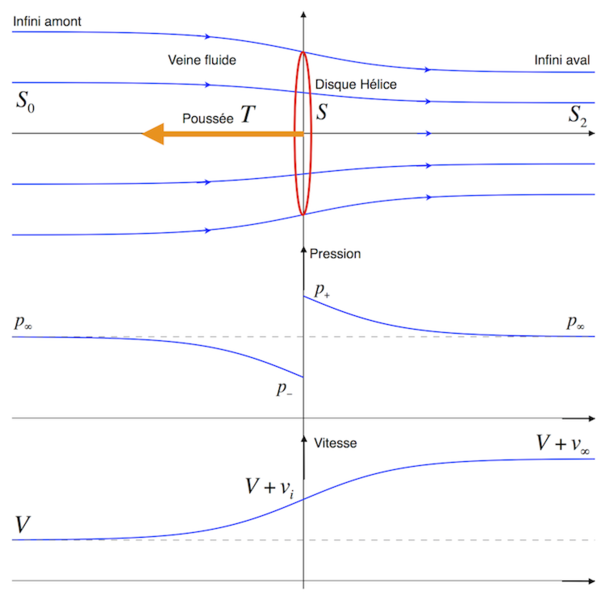
\includegraphics[width=0.6\textwidth]{FroudePropeller.png}
  \caption{Rankine-Froude theorem for propeller}
  \label{fig:rankineFroude}
\end{figure}
The rotor is represented as an idealized disk, over which a pressure
jump occurs, without a change of swirl velocity. This is at first
sight in contradiction with Euler's equation, stating that
\begin{align*}
  \power = \mFlow \Delta \fVel \aVel_u
\end{align*}
However, this idealized situation corresponds an infinite number of
blades, spinning at infinite rotation speed. Theses conditions are
approximately true for the aforementioned applications.

We distinguish four stations: (1) far upstream, ($2^-$) just before
the disk, ($2^+$) just after the disk and (3) far downstream. When the
rotor adds energy to the fluid, the latter will accelerate and the
stream tube will contract; if the rotor extracts energy, the stream
tube will expand around the rotor. We assume that
\begin{itemize}
\item the flow is incompressible and without losses;
\item far upstream and downstream the pressure is equal to the ambient
  pressure $\pres_a$; 
\item the velocity is continuous across the disk, \ie $\aVel_{2^-} =
  \aVel_{2^+} =\aVel_{2}$ due to conservation of mass;
\item there is a pressure jump across the disk $\pres_{2^+} =
  \pres_{2^-} + \Delta p_2$
\end{itemize}
The idealised flow conditions are illustrated in figure
\ref{fig:rankineFroude}.

From Bernoulli's equation we find that the total pressure is preserved
between stations $(1)$ and $(2^-)$ resp. $(2^+)$ and $(3)$.
\begin{align*}
  \pres_a + \frac{1}{2} \dens \aVel_1^2 &= \pres_{2^-} + \frac{1}{2} \dens \aVel_2^2 \\
  \pres_{2^+} + \frac{1}{2} \dens \aVel_1^2 &= \pres_a + \frac{1}{2} \dens \aVel_3^2 \\
\end{align*}
and therefore
\begin{equation}
  \begin{split}
    \Delta p_2 = \frac{1}{2} \dens \left(\aVel_3^2 - \aVel_1^2\right) 
  \end{split}
  \label{eq:froudeDiskPressure}
\end{equation}
The force exerted by the rotor on the fluid is $T = \Delta p_2 S$;
hence the conservation of momentum teaches us
\begin{align*}
  T 
  &= \mFlow \left(\aVel_3 - \aVel_1\right) \\
  &= \dens \aVel_2 S \left(\aVel_3 - \aVel_1\right)
\end{align*}
Combining both results, we find that the velocity at the disk is the
average of the up- and downstream values: 
\begin{equation}
  \aVel_2 = \frac{\aVel_1 +\aVel_3}{2}
  \label{eq:froudeDiskVelocity}
\end{equation}
Equations \ref{eq:froudeDiskPressure} and \ref{eq:froudeDiskVelocity}
allow to reconstruct the operating point - if the restrictive
hypotheses are respected.

%%%-----------------------------------------------------------------------------
\section{Actuator disk}
\label{sec:actuatorDisk}
%%%-----------------------------------------------------------------------------

%%%-----------------------------------------------------------------------------
\section{Radial equilibrium}
\label{sec:radialEquilibrium}
%%%-----------------------------------------------------------------------------


%%% Local Variables: 
%%% mode: latex
%%% TeX-master: t
%%% End: 
